\subsection{Erzeugung}
 %TODO split in 2 notes
\begin{iframe}
	\framesubtitle{Feynman-Diagramme}
	\begin{columns}
		\begin{column}{0.48\textwidth}
			\begin{figure}
				\feynmandiagram[large,horizontal=a to b] {
					i1 -- [fermion,edge label=\(e^-\)] a -- [fermion,edge label=\(e^+\)] i2,
					a -- [boson,edge label=\(\gamma\)] b,
					f1 -- [fermion,edge label'=\(\overline f\)] b -- [fermion,edge label'=\(f\)] f2,
				};
				\caption*{$e^+e^$-Vernichtung über $\gamma$ \cite{perkins}}
			\end{figure}

		\end{column}
		\begin{column}{0.48\textwidth}

			\begin{figure}
				\feynmandiagram[large,horizontal=a to b] {
					i1 -- [fermion,edge label=\(e^-\)] a -- [fermion,edge label=\(e^+\)] i2,
					a -- [boson,edge label=\(Z^0\)] b,
					f1 -- [fermion,edge label'=\(\overline f\)] b -- [fermion,edge label'=\(f\)] f2,
				};
				\caption*{$e^+e^$-Vernichtung über $Z^0$ \cite{perkins}}
			\end{figure}
		\end{column}
	\end{columns}
	\begin{figure}
		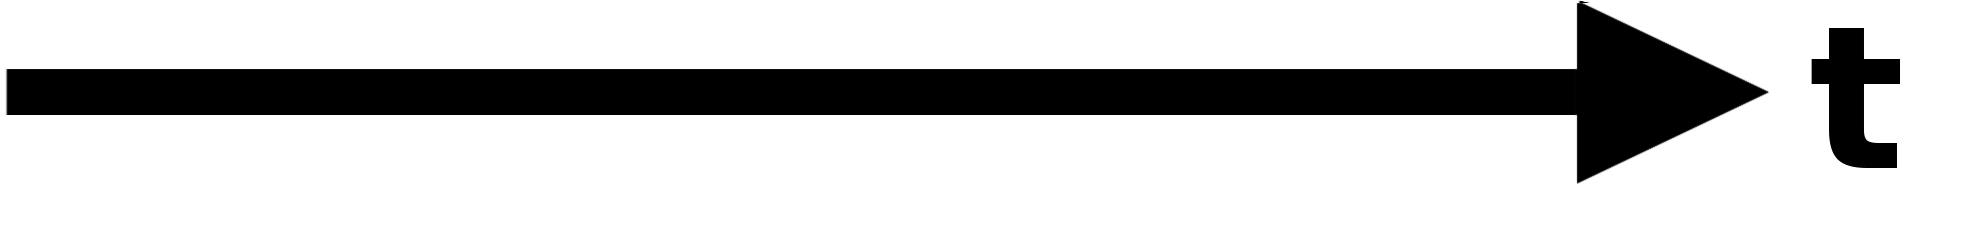
\includegraphics[height=0.25cm]{img/zeit}
	\end{figure}
\end{iframe}

\note[itemize] {
	\item W/Z-Boson durch Antilepton+Lepton/AntiQuark+Quark Reaktion
	\item kollidierende Teilchenstrahlen
	\item feynman diagram
	\item Zeit nach rechts
	\item Antiteilchen Zeitlich invers (Aus Dirac-Gleichung (Schrödinger gleichung mit eingesetzter Impuls/Energie Relation wirkt auf vier komponentigen Dirac Spinor) ergeben sich positive und negative Lösungen für die Energie) (bzw. Klein Gordon Gleichung (entkoppelt)) nach Stückelberg-Feynman-Interpretation, bsplw. E-Feld $e^-$ vs $e^+$ mit anderer Richtung ist gleich. (Dirac sagte Antiteilchen vorher/definierte, wobei negative Energien besetzt sind und Löcher sich ausbreiten basierend auf Pauli-Ausschlussprinzip, da Bosonen nicht gehorchen => reverse Zeit Interpretation)
	\item über $\gamma $oder $Z$ zu Fermion und Antifermion paar.
	\item bei passender Energie\ approx $M_Z$  dominiert $Z^0$, aus QFT+Feynmanregeln
}
%TODO check greater than kerne teilchen povh
\begin{iframe}
	\begin{itemize}
		\item LEP
		\begin{itemize}
			\item $e^-  + e^+ \rightarrow Z^0$: Schwerpunktsenergie $\sqrt{s} = 2E_e \geq M_\text{Z}c^2 \approx \SI{91.6}{GeV}$
			\item $e^+ + e^- \rightarrow W^+ + W^-$: benötigt $2E_e \geq 2M_\text{W}c^2 \approx \SI{160.8}{GeV}$
		\end{itemize}
		\pause
		\item SPS/Sp$\overline{\text{p}}$S
		\begin{itemize}
			\item $u + \overline{u} \rightarrow Z^0 $: $pp$-Kollision benötigt $E_p \gtrapprox \SI{600}{GeV}$
			\item $u  + \overline{u} \rightarrow Z^0 $: $p\overline{p}$-Kollision benötigt $E_p \gtrapprox \SI{300}{GeV}$
		\end{itemize}
	\end{itemize}
	\only<1> {
	\note[item]{ 1989 am Stanford Linear Collider und LEP}
	\note[item]{Tritt nicht auf bei Energien $\approx \SI{100}{GeV}$}
	\note[item]{ 1996 am LEP, 50 $\rightarrow$ 86 $\rightarrow$  \SI{104.6}{GeV}}
	}
	\only<2> {
	\note[item]{Energie muss in Quarks enthalten sein $\rightarrow$ sehr viel mehr Energie auf Protonen (analog mit d) => e-e+ Kollision einfacher}

	\note[item] { Besser Proton-Antiproton, da weniger Enrgie notwendig.}
	\note[item]{ in Beschleuniger inverse Rotation}
	}
\end{iframe}

\iffalse
\begin{iframe}
	\framesubtitle{Luminosität}
	\begin{equation*}
		\dot{N}_f = \sigma_f \mathcal{L}
	\end{equation*}
	\begin{figure}
		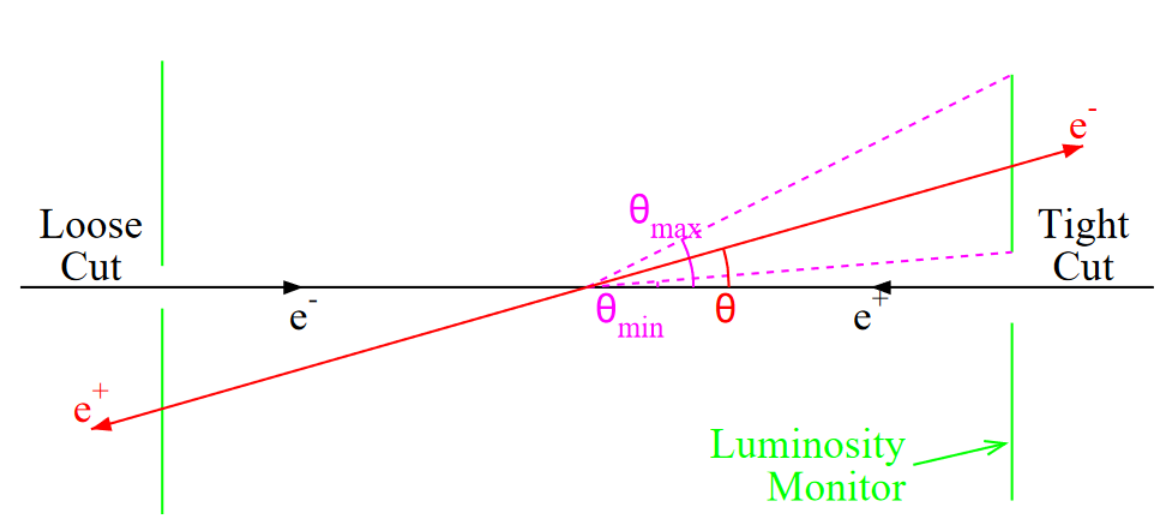
\includegraphics[height=3.5cm]{img/bhabha}
		\caption*{Bhabha Streuung \cite{huz0}}
	\end{figure}
	\note[item] {Gibt Events pro Zeit Detektion pro Wirkungsquerschnitt an.}
	\note[item]{Luminosität hängt von Beschleuniger ab}
	\note[item]{sigma ist gesucht}
	\note[item]{N sind Anzahl Teilchen be REaktion}
	\note[item]{eig. noch Fehler korrektur mit Akzeptanzraten und Effizienzen}
	\note[item]{Wirkungsquerschnitt für Bhabha-Streuung ee -> ee reine QED ziemlich genau bekannt (Kamera am detektor?)}
\end{iframe}
\fi


\begin{iframe}
\framesubtitle{Einfluss auf Beschleuniger durch Gezeiten}
\begin{figure}
		\includegraphics<1>[height=5cm]{img/gezeit}
		\includegraphics<2>[height=5cm]{img/tide}
		\only<1>{\caption*{LEP Ausdehnung\cite{cern}}}
		\only<2>{\caption*{Relative Strahlenergieänderung\cite{huz0}}}
	\end{figure}
	\only<1> {
	\note[item]{weiter relevanter Effekt}
	\note[item]{Energie schwankt im Tagesverlauf}
	\note[item]{Güne Linie ist grob Erdrotation}
	}
	\only<2> {
	\note[item]{Resonante depolarisation genaue Enrgiemessung (notwendig)} %TODO Folie?
	\note[item]{Über Verhalten des Spins der beschleunigten Elektronen}
	\note[item]{Größe primär relevant für Energie (+Synchrotron strahlung)}
	}
\end{iframe}

\subsection{Nachweis}
\begin{iframe}
\framesubtitle{durch neutrale Ströme}
	\begin{columns}
		\begin{column}{0.59\textwidth}
			\begin{figure}
				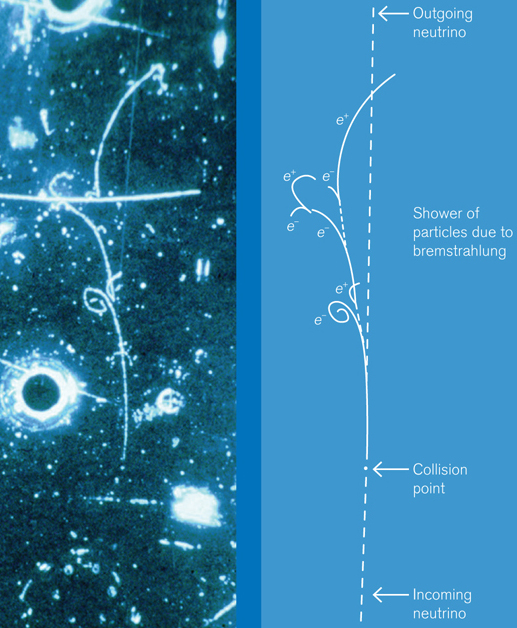
\includegraphics[width=6.7cm]{img/neutralerstrom}
			\end{figure}
		\end{column}
		\begin{column}{0.39\textwidth}
			\begin{itemize}
				\item Neutrinostrahl durch $\pi^+ \rightarrow \mu^+ + \overline{\nu}_\mu $
				\item Blasenkammer: $\bar{\nu}_\mu + e^- \rightarrow \bar{\nu}_\mu + e^-$
				\item Elektron sendet Bremsstrahlung aus
				\item $e^-e^+$-Paarbildung $\rightarrow$ elektromagnetischer Schauer
			\end{itemize}
			{\small
			 \cite{HASERT1973121}\cite{sym}}
		\end{column}
	\end{columns}

\note[item]{Striche und Kreise sind Lamben und Spiegel Reflexionen}
\note[item]{Myonlose Neutrinoreaktion}
\note[item]{Neutrale Ströme von links nach rechts Antineutrinostrahl in Blasenkammer.}
\note[item]{Neutrionstrahl durch bsplw. $\pi^+ \rightarrow \mu^+ + \overline{\nu}_\mu $ und Ladungsfilter}
\note[item]{Photon nur bei elektr. Prozessen.(=> neutraler Strom, Z)}
\note[item]{Vorhergesagter Winkel und 1/3 Energie des $e^-$ impliziert Wechselwirkung durch neutrale Ströme. }
\note[item]{700000 - Bilder überprüft. Spiral/Bremsstrahlung. }
\end{iframe}

\begin{iframe}
	\framesubtitle{Entdeckung des $Z^0$ Bosons}
	\begin{columns}
		\begin{column}{0.48\textwidth}
			\begin{figure}
				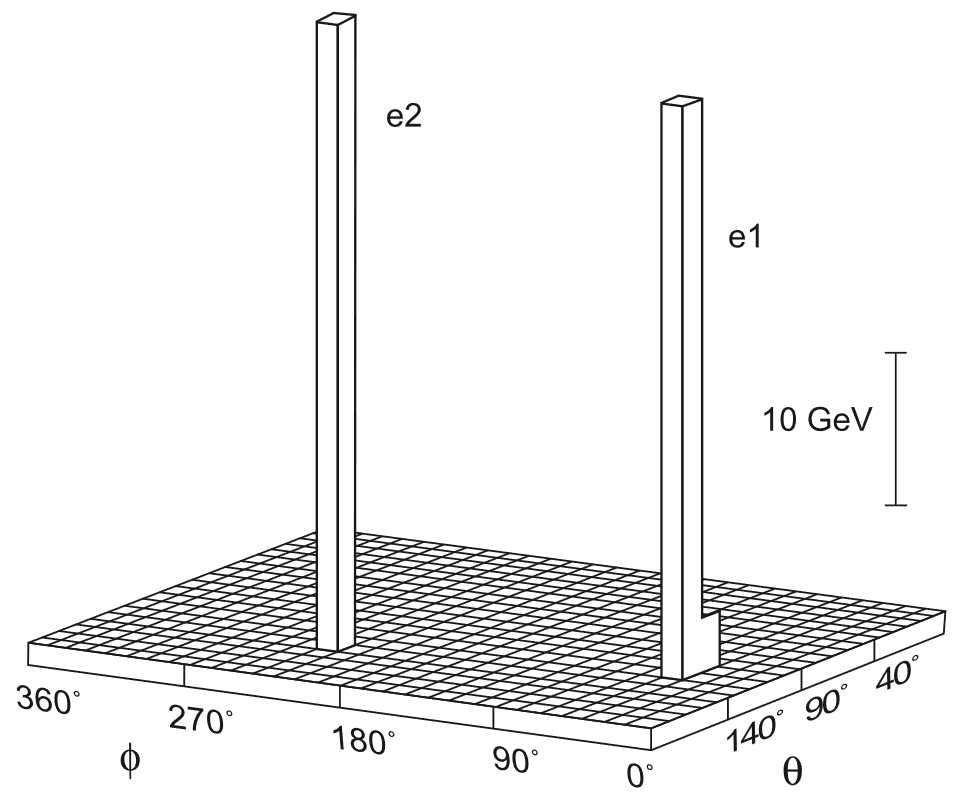
\includegraphics[width=5cm]{img/lego}
				\caption*{"Lego-Diagramm" $q+\overline{q} \rightarrow Z^0 \rightarrow e^+ + e^-$ \cite{povh}}
			\end{figure}
		\end{column}
		\begin{column}{0.48\textwidth}
				\begin{itemize}
					\item 1983 UA2 Detektor am Sp$\overline{\text{p}}$S
					\item Masse des $Z^0$-Bosons entspricht der Summe der Energie von $e^-$ und $e^+$
					\item Entgegengesetzte Impulse von $e^-$ und $e^+$
				\end{itemize}
		\end{column}
		\end{columns}
\end{iframe}

\note[itemize] {
	\item nicht L3, aber analog
	\item Beispiel Event einer der ersten Messung
	\item Plane unten sind Kaloriemeterzellen
	\item Energie Summe $=$ Masse $Z^0$
	\item Winkel 180° => entgegen gesetzte Richtungen

	%\item ?Woher sicher, dass $Z^0$ Zerfall? %TODO
}

%TODO andere GRaphiken für Jet+ee
\subsection{Präzisionsmessungen}
\begin{iframe}
	\framesubtitle{Large Electron Positron Collider (LEP, 1989-2000)}
	\begin{figure}
		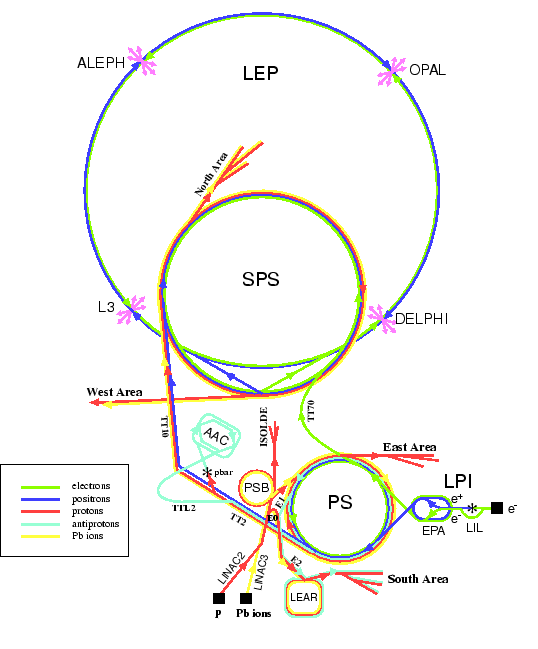
\includegraphics[height=5cm]{img/lep}
		\caption*{Beschleuniger am CERN 1996 \cite{lepacc}}
	\end{figure}
	\note[item] { LEP wurde zu LHC}
	\note[item] { L3 wurde zu ALICE}
	\note[item] { SppS von 1981 bis 1991 anstelle von SPS}
	\note[item] { Erzeugung, Lineare Beschleuniger und Vorstufen }
\end{iframe}

\begin{iframe}
	\framesubtitle{L3 Detektoraufbau am LEP}
	\begin{columns}
	\begin{column}{0.49\textwidth}
\begin{figure}
		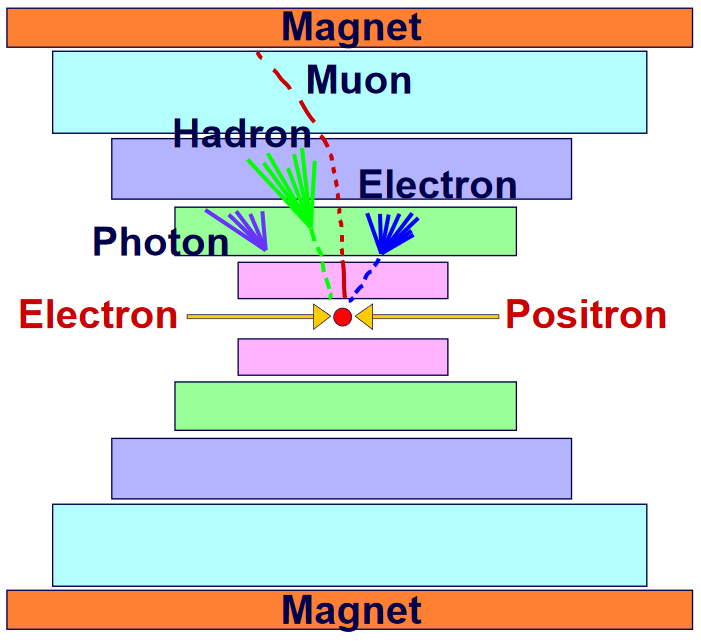
\includegraphics[height=4.5cm]{img/skizze}
		\caption*{L3 Detektor \cite{huz0}}
	\end{figure}
\end{column}
	\begin{column}{0.49\textwidth}
		Von Innen nach Außen:
		\begin{enumerate}
			\item Spurdetektor
			\item Elektromagnetisches Kalorimeter
			\item Hadronisches Kalorimeter
			\item Myonkammer
		\end{enumerate}
\end{column}
\end{columns}
	%\note[item]{Analog Vorlesung, Hadronen Jets}
	%\note[item]{Masse/Ladung durch Felder+ Drifts mit Magnetfeld}
	\note[item]{Alles in Magnetfeld}
	\note[item]{Spurdetektor: misst elektrische Teilchen}
	\note[item]{Krümmung gibt Impuls und Ladung}
	\note[item]{EM Kalorimeter: Energie von Elektron und Photon, EM Teilchen wird absorbiert}
	\note[item]{Had Kalorimeter: Energie von Hadronen, starke WW Teilchen werden absorbiert}
	\note[item]{Myonkammern: Für Myonen, groß, weil geringe WW}
	\note[item]{Vortrag speziell zur Teilchendetektion}
\end{iframe}

\begin{iframe} %TODO notwendig?
	\framesubtitle{L3 Detektoraufbau am LEP}
	\begin{columns}
	\begin{column}{0.49\textwidth}
\begin{figure}
		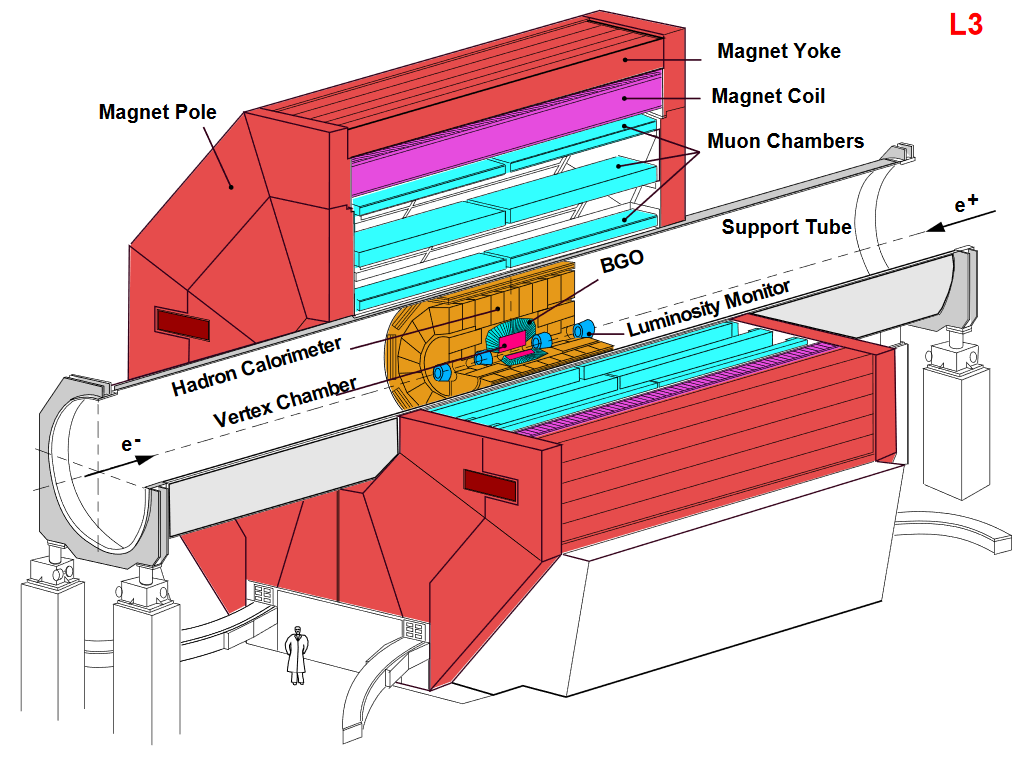
\includegraphics[height=4.0cm]{img/detektor}
		\caption*{L3 Detektor \cite{huz0}}
	\end{figure}
\end{column}
	\begin{column}{0.49\textwidth}
\end{column}
\end{columns}
	\note[item]{Mensch für Größenverhältnis.}
	\note[item]{Magnet im ALICE wieder verwendet.}
\end{iframe}



\begin{iframe}
	\framesubtitle{L3 Detektor (1993 am LEP)}
	\begin{columns}
		\begin{column}{0.40\textwidth}
	\begin{figure}
		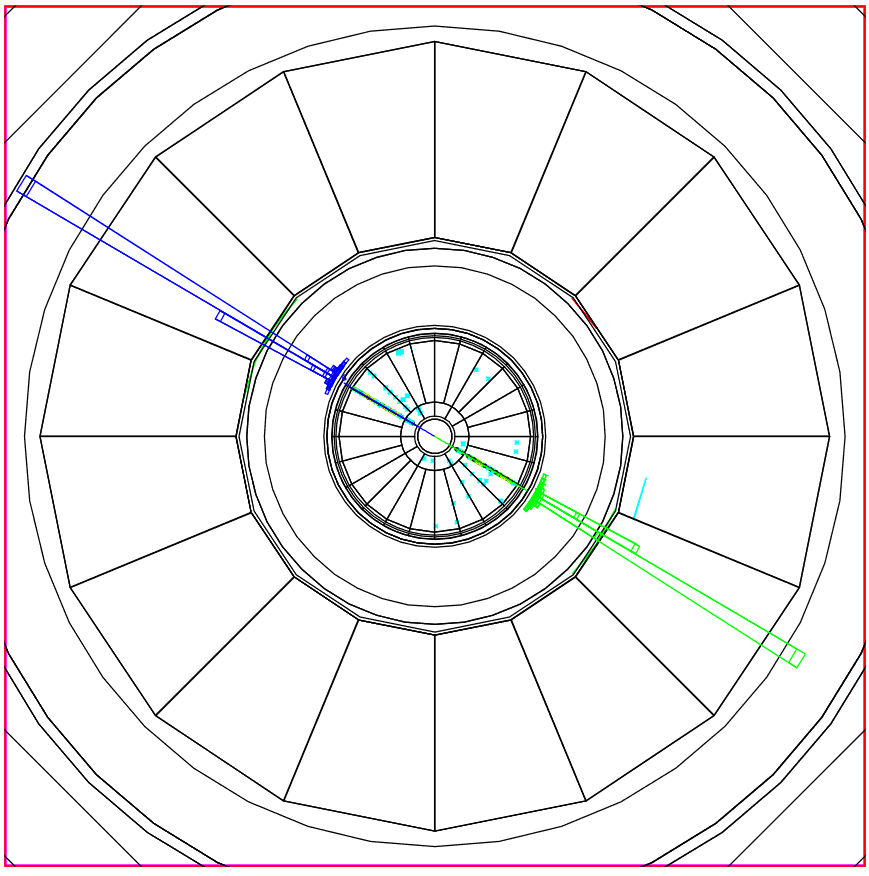
\includegraphics[height=4.70cm]{img/elektron}
		\caption*{$e^- +e^+ \rightarrow Z^0 \rightarrow e^- + e^+$ \cite{huz0}}
	\end{figure}
\end{column}
		\begin{column}{0.58\textwidth}
			\begin{itemize}
				\item Energiemessung im elm. Kalorimeter
				\item Entgegengesetzte Ausbreitung
			\end{itemize}
\end{column}
\end{columns}

\note[item]{ L3 Detektor LEP}
	\note[item]{beispielhafte Ereignisse}
	\note[item]{entlang der Strahlachse}
	\note[item]{ analog zu Lego}
	\note[item]{ herausgezoomt, weil Enrgie weniger verteilt}
	\note[item]{ Winkel 180° => entgegen gesetzte Richtungen}
	\note[item]{Balken sind die Energien die Kaloriemeter messen}
	%\note[item]{?Woher sicher, dass $Z^0$ Zerfall?} %TODO
	%\note[item]{?Wie tauon detektieren?} %TODO
\end{iframe}

\begin{iframe}
	\framesubtitle{L3 Detektor (1993 am LEP)}

\begin{columns}
		\begin{column}{0.40\textwidth}
	\begin{figure}
		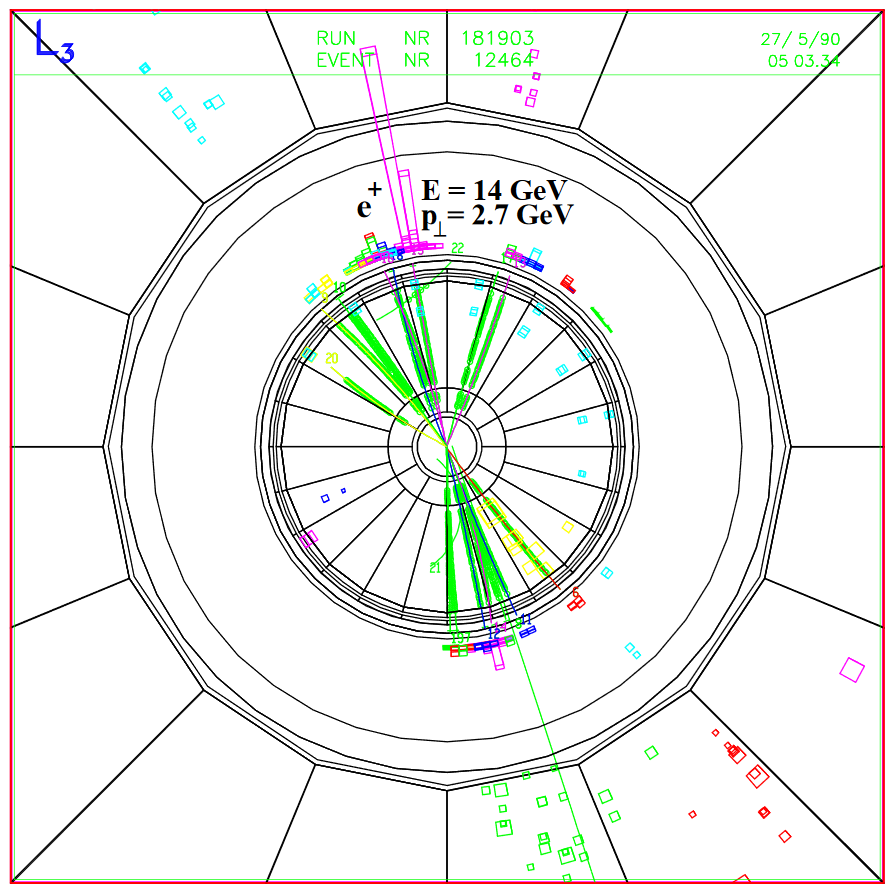
\includegraphics[height=4.70cm]{img/hadron}
		\caption*{$e^- +e^+ \rightarrow Z^0 \rightarrow$ hadronische Jets \cite{huz0}}
	\end{figure}
\end{column}
		\begin{column}{0.58\textwidth}
			\begin{itemize}
				\item Einzelnes Quark führt zu Quark-Antiquark-Paar Erzeugung, um isolierte Farbladung zu verhindern (Confinement)
				\item Reaktion äußert sich in hadronische Jets
				\item Energiemessung im Hadronischen Kalorimeter
			\end{itemize}
\end{column}
\end{columns}
		\note[item]{ Hadronische Jets, Farbladung nicht aleine vorkommend, immmer neue Quark-Antiquark-Paare (Confinment)}
\end{iframe}

\begin{iframe}
	\framesubtitle{L3 Detektor (1993 am LEP)}

\begin{columns}
		\begin{column}{0.40\textwidth}
	\begin{figure}
		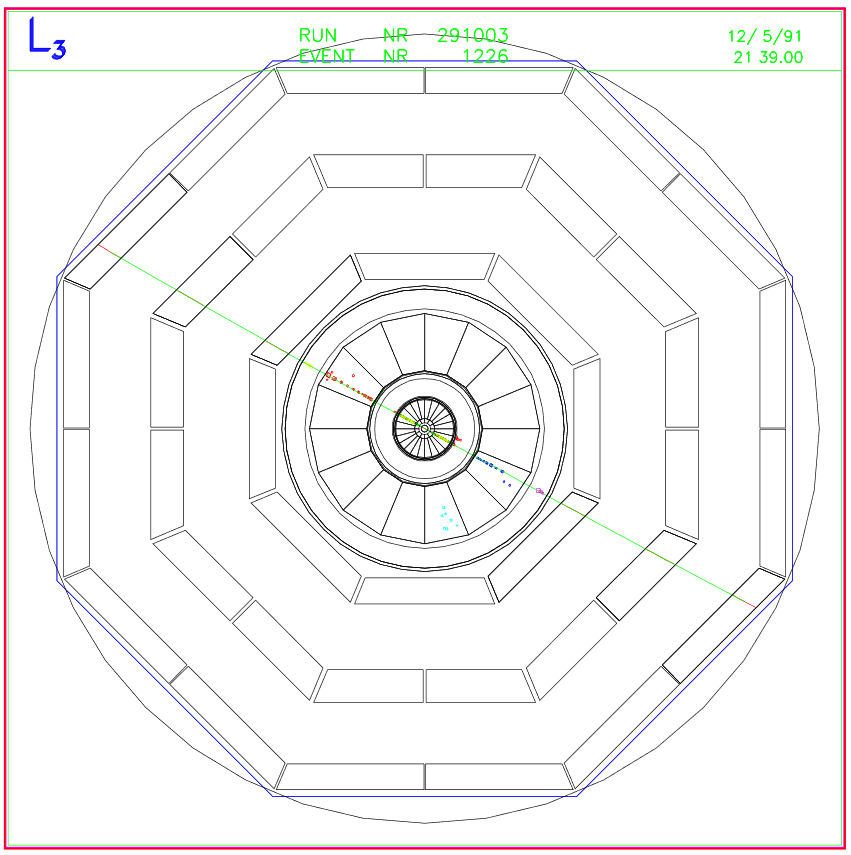
\includegraphics[height=4.70cm]{img/muon}
		\caption*{$e^- +e^+ \rightarrow Z^0 \rightarrow \mu^+ + \mu^-$ \cite{huz0}}
	\end{figure}
\end{column}
		\begin{column}{0.58\textwidth}
			\begin{itemize}
				\item Messung der Spur der Myonen durch mehrere Myonkammern
				\item I.A. keine Absorption
			\end{itemize}
\end{column}
\end{columns}
		\note[item]{Muon erst an äußeren Platten detektiert}
\end{iframe}

\begin{iframe}
	\begin{columns}
		\begin{column}{0.49\textwidth}
	\begin{figure}
		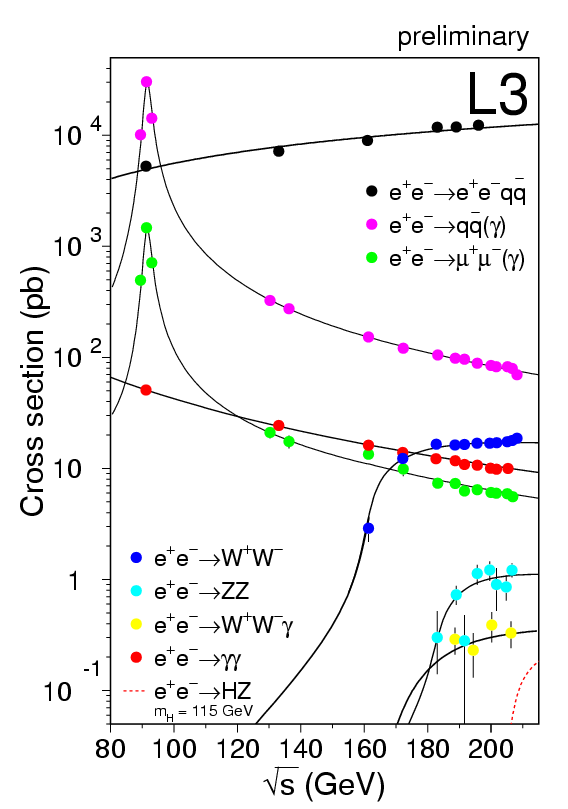
\includegraphics[height=5cm]{img/l3wirk}
		\caption*{Wirkungsquerschnitte bei $e^-e^+$ Kollision \cite{l3hp}}
	\end{figure}
\end{column}
		\begin{column}{0.49\textwidth}
			\begin{itemize}
				\item $Z^0$ Resonanz bei $\approx \SI{91}{GeV}$
			\end{itemize}
\end{column}
\end{columns}
	\note[item] {Achsen + Farbliche Zuordnung}
	\note[item] {$Z^0$ Resonanz und weitere Messungen}
\end{iframe}

\subsection{Eigenschaften}
\begin{iframe}
	\framesubtitle{Experimentelle Bestimmung}
	\begin{itemize}
		\item Messung: %TODO Graphik!!
		\begin{itemize}
			\item $M_Z = \SI{91.188+-0.002}{GeV/c^2}$
			\item $\Gamma_Z = \SI{2.495+-0.002}{GeV}$
		\end{itemize}
		\pause
		\item Zerfall:
		\begin{align*}
			Z^0 \rightarrow & e^- + e^+ & \SI{3.363+-0.004}{\%} \\
			& \mu^- + \mu^+ & \SI{3.366+-0.007}{\%} \\
			& \tau^- + \tau^+ & \SI{3.370+-0.008}{\%} \\
			& \nu_{e,\mu,\tau} + \overline{\nu}_{e,\mu,\tau} & \SI{20+-0.06}{\%} \\
			& \text{Hadronen} & \SI{69.91+-0.06}{\%} \\ %TODO Align
		\end{align*}
	\end{itemize}
	\only<1> {
		\note[item]{Über Wirkungsquerschnitt? src [PD12]}
		\note[item]{Breite + Maximalstelle} %TODO
	}
	\only<2> {
		\note[item]{Hadronen (idR. Anti+Quark) nicht unterscheidbar} %TODO Ladungsunterscheidung?
		\note[item]{Anti+Neutrino schwer detektierbar => \% über $\Gamma_\text{tot}$}
}
%\note[item]{totale Breite = alle Zerfälle Anti+Fermion???} %TODO
%\note[item]{$Z^0$ nicht nur ungeladenes $W$-Boson, da }
\end{iframe}

\subsection{Anzahl Neutrinogenerationen}

\begin{iframe}
	\framesubtitle{Wirkungsquerschnitt}
	\begin{columns}
		\begin{column}{0.48\textwidth}
			\begin{equation*}
				\sigma_f \propto  \frac{\Gamma_f\cdot \Gamma_e}{(s-M_Z^2)^2 + M_Z^2\Gamma_Z^2}
			\end{equation*}
		\end{column}
		\begin{column}{0.48\textwidth}
		\end{column}
	\end {columns}
	\begin{textblock*}{5cm}(7cm,3cm) % {block width} (coords)
				\begin{figure}
				\feynmandiagram[large,horizontal=a to b] {
					i1 -- [fermion,edge label=\(e^-\)] a -- [fermion,edge label=\(e^+\)] i2,
					a -- [boson,edge label=\(Z^0\)] b,
					f1 -- [fermion,edge label'=\(\overline f\)] b -- [fermion,edge label'=\(f\)] f2,
				};
			\end{figure}
		\end{textblock*}
\note[item]{Formel für $\sigma$ Breit-Wigner}
\note[item]{Einheiten $h$ und $c$ multiplizieren}
\note[item]{Abhängig von ...}
\note[item]{$\gamma$ unterdrückt}
\end{iframe}

\begin{iframe}
	\framesubtitle{Zerfallsbreite}
	\only<3> {
	\begin{textblock*}{5cm}(6.5cm,2.4cm) % {block width} (coords)
	\begin{equation*}
		\Gamma_f=\frac{G_F M_Z^3}{24\sqrt{2}\pi}\cdot (1+(1-e|Q_f|\sin^2{\theta_W})^2)
	\end{equation*}
	\end{textblock*}
	}
	\only<4> {
	\begin{textblock*}{5cm}(6.5cm,2.4cm) % {block width} (coords)
	\begin{equation*}
		\Gamma_f=\frac{G_F M_Z^3}{24\sqrt{2}\pi}\cdot (1+(1-e|Q_f|\sin^2{\theta_W})^2)
	\end{equation*}
	\end{textblock*}
	}
	\only<5> {
	\begin{textblock*}{5cm}(6.5cm,2.4cm) % {block width} (coords)
	\begin{equation*}
		\Gamma_f=\frac{G_F M_Z^3}{24\sqrt{2}\pi}\cdot (1+(1-e|Q_f|\sin^2{\theta_W})^2)
	\end{equation*}
	\end{textblock*}
	}
	\only<6> {
	\begin{textblock*}{5cm}(6.5cm,2.4cm) % {block width} (coords)
	\begin{equation*}
		\Gamma_f=\frac{G_F M_Z^3}{24\sqrt{2}\pi}\cdot (1+(1-e|Q_f|\sin^2{\theta_W})^2)
	\end{equation*}
	\end{textblock*}
	}
	\begin{align*}
		\action<+->{\Gamma_Z&=\sum_f \Gamma_{Z \rightarrow f\bar{f}}\\}
		\action<+->{&= \Gamma_\text{u,c,d,s,b}  + \Gamma_\text{e,$\mu$,$\tau$}+ \Gamma_{\nu_e,\nu_\mu,\nu_\tau}\\}
		\action<+->{&= N_C \cdot2\cdot\Gamma_u + N_C\cdot 3\cdot \Gamma_d + 3\cdot\Gamma_e + N_\nu \cdot\Gamma_\nu\\}
		\action<+->{&= 3 \cdot 2\cdot\SI{94.9}{MeV} + 3\cdot3\cdot \SI{122.4}{MeV}+ 3\cdot \SI{83.3}{MeV} + 3\cdot \SI{165.8}{MeV} \\}
		\action<+->{&=\SI{2.42}{GeV}\\}
		\action<+->{&\xrightarrow[\text{korrektur}]{\text{Strahlungs-}}\SI{2.497}{GeV}\\}
	\end{align*}
	\only<1> {
		\note[item] {Breite ergibt sich aus Partial Breiten}
	}
	\only<2> {
		\note[item] { kein top-Quark, da t-Masse ($\approx \SI{175}{ GeV}$)größer als $Z^0$-Masse ist}
	}
	\only<3> {
		\note[item]{$\Gamma_f=\frac{G_F M_Z^3}{24\sqrt{2}\pi}\cdot (1+(1-e|Q_f|\sin^2{\theta_W})^2)$}
		\note[item]{$G_F$ Fermikonstante}
		\note[item]{$Q_f$ Ladung des Fermions}
		\note[item]{Quantenmechanisch Herleitung der Formel nicht notwendig}
		\note[item]{primär von Ladung abhängig}
		\note[item]{ Lep: $e^\pm$, $\mu^\pm$, $\tau^\pm$}
		\note[item]{ Had: u,c= 2/3; d,s,b=-1/3}
		\note[item]{ Neutrinos}
		\note[item] { $N_C$ Anzahl Farbledungsnmöglichkeiten}
		}
		\only<4> {
		\note[item]{Einsetzen, vgl Maximal für minimale Ladung}
		}
		\only<5> {
		\note[item] { Summe}
		}
		\only<6> {
		\note[item]{Korrekturen aus QFT, höherer Ordungen, Strahlungskorrektur}
		\note[item]{Passt mit Unsicherheiten zu Exp. (nicht auf Folie)}
		\note[item]{$\Gamma_e/\Gamma_{tot}=3,37\%$ passt auch zu Exp.}
		}
\end{iframe}

\begin{iframe}
	\framesubtitle{Vergleich Theorie und Experiment}

	%\begin{table}
		\centering
		\begin{tabular}{| c | c | c |}
			\hline
			  $Z^0$ Zerfall&  theoretisch& experimentell\\ \hline
				$e^-+e^+$& \SI{3.34}{\%}& \SI{3.363(4)}{\%}\\
				$\nu+\overline{\nu}$&\SI{19.92}{\%} & \SI{20.0(6)}{\%}\\
				Hadronen& \SI{66.92}{\%} & \SI{69.91(6)}{\%}\\
				\hline
				\hline
				$\Gamma_Z$ & \SI{2.497}{GeV} & \SI{2.495(2)}{GeV}\\
				\hline
		\end{tabular}
	%\end{table}
	\note[item]{$e^-$ exemplarisch für Leptonen}
	\note[item]{passt alles gut}
\end{iframe}

\begin{iframe}
	\begin{columns}
		\begin{column}{0.48\textwidth}
	\begin{figure}
		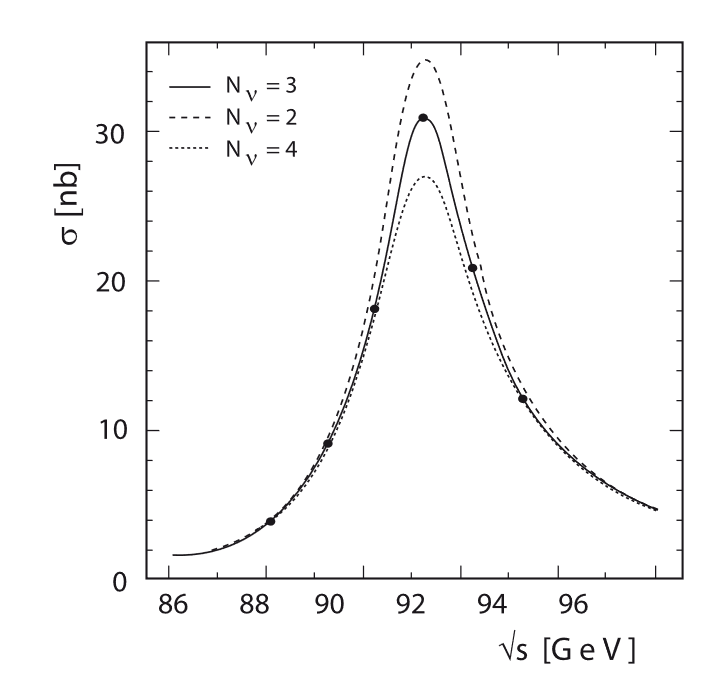
\includegraphics[width=5.4cm]{img/neutrinogen}
		\caption*{Wirkungsquerschnitt $e^+e^-\rightarrow $Hadronen \cite{povh}}
	\end{figure}
\end{column}
		\begin{column}{0.48\textwidth}
			\begin{itemize}
				\item OPAL-Detektor am LEP
				\item 3 Neutrinogenerationen passen zu Messungen
				\item Hinweis für 3 Generationen von Leptonen und Quarks
			\end{itemize}
		\end{column}
\end{columns}
	\note[item]{Cern Experiment}
	\note[item]{Wirkungsquerschnitt gegen Schwerpunktenergie  }
	\note[item]{Ähnlich der Breit Wigner Funktion aber nicht passend symmetrisch durch Korrekturen höherer Ordnung udn Bremstrahlung durch $e^-$}
	\note[item]{Verschiedene Anzahl-Neutrinogenerationen-Kurven}
	\note[item]{3 Neutrinogenerationen $\rightarrow$ 3 Leptonen 3 Quarks Generationen}
\end{iframe}
%TODO Neutrino generationen
